\documentclass[11pt,letterpaper]{article}
\usepackage{lac2012}
\usepackage[utf8]{inputenc}
\usepackage{color}
\usepackage{graphicx}
\usepackage{hyperref}
\definecolor{mycolor}{rgb}{0.384,0.0,0.145}
\hypersetup{
	colorlinks=true,
	linkcolor= mycolor,
	citecolor= mycolor
}

\sloppy
\newenvironment{contentsmall}{\small}

\newcommand{\inscore}		{\textsc{\small INScore}}
\newcommand{\lra}			{$\leftrightarrow$}
\newcommand{\rshift}		{\hspace*{11mm}}
\newcommand{\roshift}		{\hspace*{8mm}}
\newcommand{\OSC}[1]		{\texttt{#1}}

\hyphenation{INScore}

\definecolor{mygrey}{gray}{0.92}
\newcommand{\map}	[1]			{\colorbox{mygrey}{
								\begin{minipage}[t]{0.95\columnwidth} 
								\begin{contentsmall}
								{\texttt{#1}}
								\end{contentsmall}
								\end{minipage}
								}}


\title{\textsc{{\LARGE INScore}} \\
{\Large \textbf{An Environment for the Design of Live Music Scores}}
}

%see lac2012.sty for how to format multiple authors!
\author
{D. Fober \and Y. Orlarey \and S. Letz
\\ Grame - Centre national de création musicale 
\\ 9, rue du Garet BP 1185 
\\ 69202 Lyon Cedex 01,
\\ France, 
\\ \{fober, orlarey, letz\}@grame.fr
}




\begin{document}
\maketitle


\begin{abstract}
\begin{contentsmall}
\inscore\ is an open source framework for the design of interactive, augmented, live music scores. Augmented music scores are graphic spaces providing representation, composition and manipulation of heterogeneous and arbitrary music objects (music scores but also images, text, signals...), both in the graphic and time domains. 
\inscore\ includes also a dynamic system for the representation of the music performance, considered as a specific sound or gesture instance of the score, and viewed as \emph{signals}. 
It integrates an \emph{event based} interaction mechanism that opens the door to original uses and designs, transforming a score as a user interface or allowing a score self-modification based on temporal events. 
This paper presents the system features, the underlying formalisms, and introduces the OSC based scripting language.
\end{contentsmall}
\end{abstract}

\keywords{
\begin{contentsmall}
score, interaction, signal, synchronization
\end{contentsmall}
}

%-------------------------------------------------------------
\section{Introduction}
%-------------------------------------------------------------

Music notation has a long history and evolved through ages. From the ancient neumes to the contemporary music notation, the western culture is rich of the many ways explored to represent the music. From symbolic or prescriptive notations to pure graphic representation, the music score has always been in constant interaction with the creative and artistic process. 

However, although the music representations have exploded with the advent of computer music \cite{dann93b,hewlett01}, the music score, intended to the performer, didn't evolved in proportion to the new music forms. In particular, there is a significant gap between interactive music and the static way it is usually notated: a performer has generally a traditional paper score, plus a computer screen displaying a number or a letter to indicate the state of the interaction system. New needs in terms of music representation emerge of this context.

In the domain of electro-acoustic music, analytic scores - music scores made \emph{a postériori}, become common tools for the musicologists but have little support from the existing computer music software, apart the approach proposed for years by the Acousmograph \cite{ACOUSM04}. 

In the music pedagogy domain and based on a mirror metaphor, experiments have been made to extend the music score in order to provide feedback to students learning and practicing a traditional music instruments \cite{Fober:07b}. This approach was based on an extended music score, supporting various annotations, including performance representations based on the audio signal, but the system was limited by a monophonic score centered approach and a static design of the performance representation.

Today, new technologies allow for real-time interaction and processing of musical, sound and gestural information. But the symbolic dimension of the music is generally excluded from the interaction scheme.

\inscore\ has been designed in answer to these observations. It is an open source framework\footnote{\url{http://inscore.sf.net}} for the design of interactive, augmented, live music scores. It extends the traditional music score to arbitrary heterogeneous graphic objects: it supports symbolic music notation (Guido \cite{hoos98} or MusicXML \cite{good01} format), text (utf8 encoded or html format), images (jpeg, tiff, gif, png, bmp), vectorial graphics (custom basic shapes or SVG), video files, as well as an original performance representation system \cite{Fober:10c}.

Each component of an augmented score has a graphic and temporal dimension and can be addressed in both the graphic and temporal space. A simple formalism, is used to draw relations between the graphic and time space and to represent the time relations of any score components in the graphic space. Based on the graphic and time space segmentation, the formalism relies on simple mathematical relations between segments and on relations compositions. We talk of \emph{time synchronization in the graphic domain} \cite{fober:10b} to refer to this specific feature.

\inscore\ is a message driven system that makes use of the Open Sound Control [OSC] \footnote{\url{http://opensoundcontrol.org/}} format. This design opens the door to remote control and to interaction using any OSC capable application or device. In addition, it includes interaction features provided at score component level by the way of \emph{watchable events}. 

All these characteristics make \inscore\ a unique system in the landscape of music notation or of multi-media presentation. 
The next section gives details about the system features, including the underlying formalisms. Next the OSC API is introduced with a special emphasis on how it is turned into a scripting language. The last section gives an overview of the system architecture and dependencies before some directions are presented for future work.


%-------------------------------------------------------------
\section{Features}
%-------------------------------------------------------------

Table \ref{tblrsrc} gives the typology of the graphic resources supported by the system.
All the score elements have graphic properties (position, scale, rotation, color, etc.) and time properties as well (date and duration).

\begin{table*}[htdp]
\begin{center}
\begin{tabular}{|r|l|}
\hline 
Symbolic music description 	& Guido Music Notation and MusicXML formats \\
Text 			& plain text or html (utf8)\\
Images 			& jpg, gif, tiff, png, bmp \\
Vectorial graphics	 	&  line, rectangle, ellipse, polygon, curve, SVG code \\
Video files	& using the phonon plugin \\
Performance representations & see section \ref{perf} \\
\hline
\end{tabular}
\end{center}
\caption{Graphic resources supported by the system.}
\label{tblrsrc}
\end{table*}

INScore provides a message based API to create and control the score elements, both in the graphic and time spaces. The Open Sound Control [OSC] protocol is used as basis format for these messages, described in section \ref{osc}.

%-------------------------------------------------------------
\subsection{Time to graphic relations}
\label{mappings}
All the elements of a score have a time dimension and the system is able to graphically represent the time relationships of these elements. \inscore\ is using segmentations and \emph{mappings} to achieve this \emph{time synchronization in the graphic domain}.

The segmentation of a score element is a set of segments included in this element. A segment may be viewed as a portion of an element. It could be a 2D graphic segment (a rectangle), a time interval, a text section, or any segment describing a part of the considered element in its \emph{local} coordinates space.

Mappings are mathematical relations between segmentations. A composition operation is used to relate the graphic space of two arbitrary score elements, using their relation to the time space. 
Table \ref{maptable} lists the segmentations and mappings used by the different component types. Mappings are indicated by arrows (\lra). Note that the arrows link segments of different types. Segmentations and mappings in  \textit{italic} are automatically computed by the system, those in \textbf{bold} are user defined. 


\begin{table*}[ht]
\begin{center}
\begin{tabular}{|r|l|}
\hline
type & segmentations and mappings required \\
\hline
Symbolic music description		& \textit{graphic \lra\ wrapped time} \lra\ \textit{time} \\
Text		& \textit{graphic} \lra\ \textbf{text  \lra\ time} \\
Images		& \textit{graphic} \lra\ \textbf{pixel \lra\ time} \\
Vectorial graphics	&  \textit{graphic} \lra\ \textbf{vectorial \lra\ time} \\
Performance representations		&  \textit{graphic} \lra\ \textbf{frame \lra\ time} \\
\hline
\end{tabular}
\end{center}
\caption{Segmentations and mappings for each component type}
\label{maptable}
\end{table*}


Note that for music scores, an intermediate time segmentation, the \emph{wrapped time}, is necessary to catch repeated sections and jumps (to sign, to coda, etc.).

\begin{figure}[h]
\begin{center}
	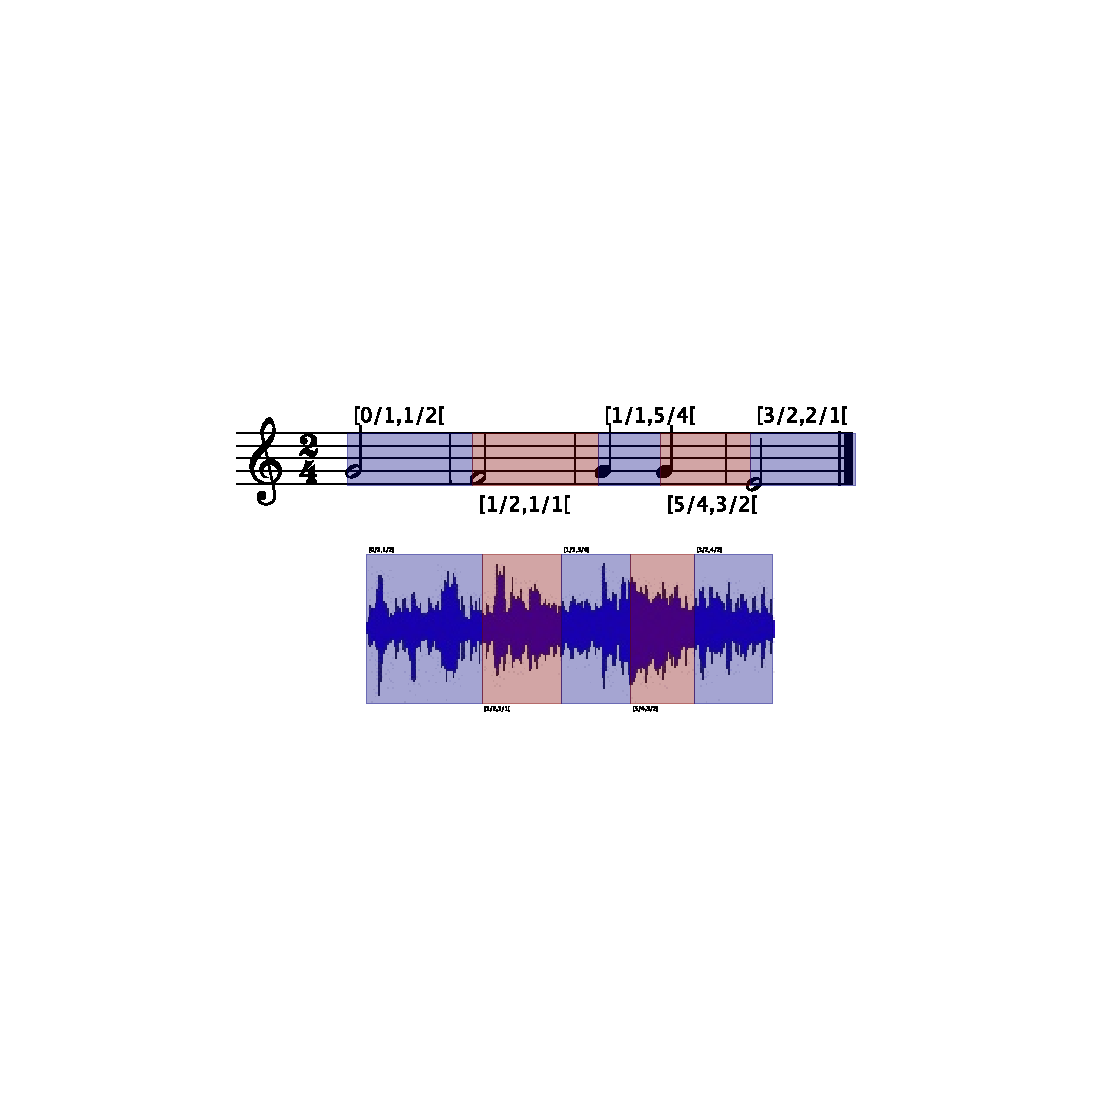
\includegraphics[width=0.98\columnwidth]{rsrc/segmentation}
\caption{Graphic segments of a score and its performance displayed using colors and annotated with the corresponding time segments.}
\label{fig:segm}
\end{center}
\end{figure}

Figure \ref{fig:segm} shows segments defined on a score and an image, annotated with the corresponding time segments. Synchronizing the image to the score will stretch and align the graphic segments corresponding to similar time segments as illustrated by figure \ref{fig:sync}.

\begin{figure}[h]
\begin{center}
	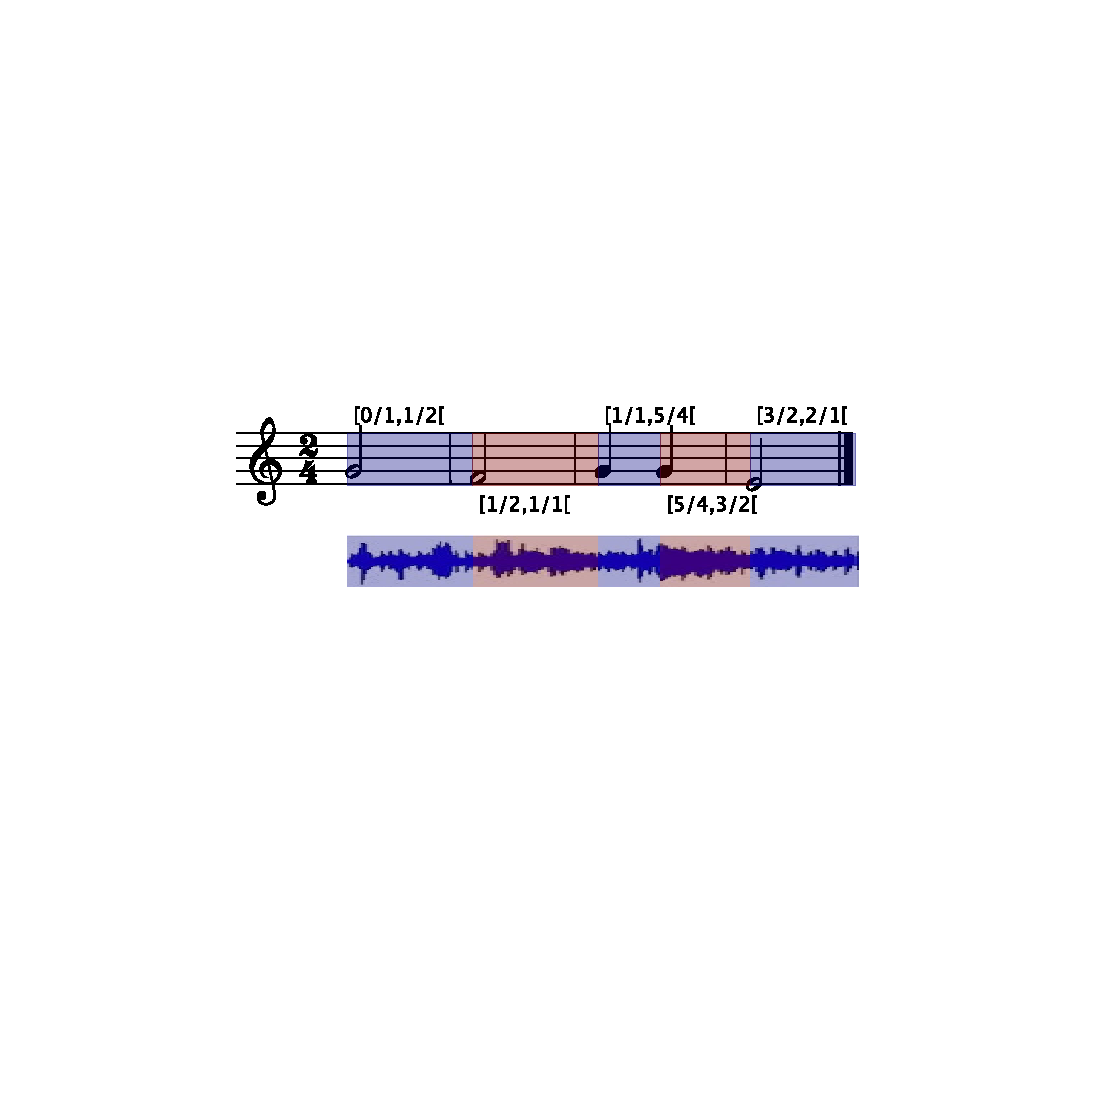
\includegraphics[width=0.98\columnwidth]{rsrc/sync}
\caption{Time synchronization of the segments displayed in figure \ref{fig:segm}.}
\label{fig:sync}
\end{center}
\end{figure}

Description of the image graphic to time relation is given in table \ref{mapex} as a set of pairs including a graphic segment defined as 2 intervals on the x and y axis, and a time segment defined as 2 rationals expressing musical time (where 1 represents a whole note).

\begin{table}[ht]
\begin{contentsmall}
\begin{center}
\begin{tabular}{l l}
( [0, 67[    [0, 86[ )	& ( [0/2, 1/2[ ) \\
( [67, 113[  [0, 86[ )	& ( [1/2, 1/1[ ) \\
( [113, 153[ [0, 86[ )	& ( [1/1, 5/4[ ) \\
( [153, 190[ [0, 86[ )	& ( [5/4, 3/2[ ) \\
( [190, 235[ [0, 86[ )	& ( [3/2, 4/2[ )
\end{tabular}
\end{center}
\end{contentsmall}
\caption{A mapping described as a set of relations between graphic and time segments.}
\label{mapex}
\end{table}


%-------------------------------------------------------------
\subsection{Performance representation}
\label{perf}

Music performance representation is based on signals, whether audio or gestural signals. To provide a flexible and extensible system, the graphic representation of a signal is viewed as a \emph{graphic signal}, i.e. as a composite signal made of:
\begin{itemize}
\item a $y$ coordinate signal
\item a thickness signal $h$
\item a color signal $c$
\end{itemize}
Such a composite signal (see figure \ref{fig:sig}) includes all the information required to be drawn without additional computation.

\begin{figure}[h]
\begin{center}
	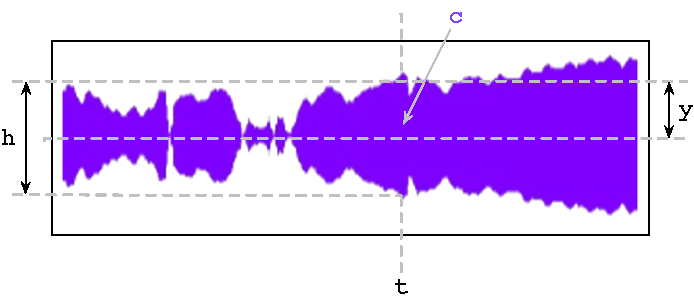
\includegraphics[width=0.98\columnwidth]{rsrc/graph}
\caption{A composite \emph{graphic signal} at time $t$.}
\label{fig:sig}
\end{center}
\end{figure}

The following examples show some simple representations defined using this model.
 
%-----------------------------------
\subsubsection{Pitch representation}
Represents notes pitches on the y-axis using the fundamental frequency (figure \ref{fig:pitch}).
\begin{figure}[htbp]
\centerline{
	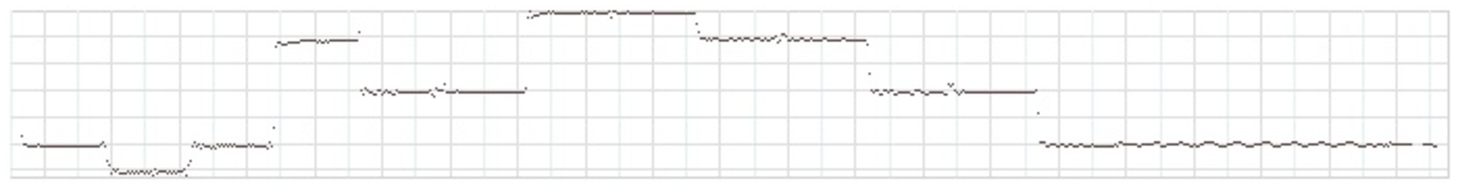
\includegraphics[width=0.99\columnwidth]{rsrc/curves/pitch}}
\caption{Pitch representation.}
\label{fig:pitch}
\end{figure}

The corresponding graphic signal is expressed as:
\[ g = S_{f0}\ /\ k_t\ /\ k_c \]
where $S_{f0}$ : fundamental frequency \\
\rshift	 $k_t$ : a constant thickness signal \\
\rshift	 $k_c$ : a constant color signal 
 
%-----------------------------------
\subsubsection{Articulations}
Makes use of the signal RMS values to control the graphic thickness
(figure \ref{fig:articulation}).
\begin{figure}[htbp]
\centerline{
	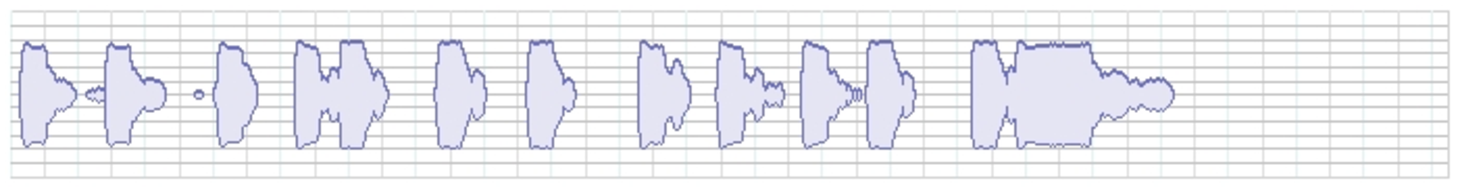
\includegraphics[width=0.99\columnwidth]{rsrc/curves/articulation}}
\caption{Articulations.}
\label{fig:articulation}
\end{figure}
The corresponding graphic signal is expressed as:
\[ g = k_y\ /\ S_{rms}\ /\ k_c \]
where $k_y$ : signal $y$ constant \\
\rshift	 $S_{rms}$ : RMS signal \\
\rshift	 $k_c$ : a constant color signal 
 
%-----------------------------------
\subsubsection{Pitch and articulation combined}
\label{pitchart}
Makes use of the fundamental frequency and RMS values to draw articulations shifted by the pitches
(figure \ref{fig:pitchedarticulation}).
\begin{figure}[htbp]
\centerline{
	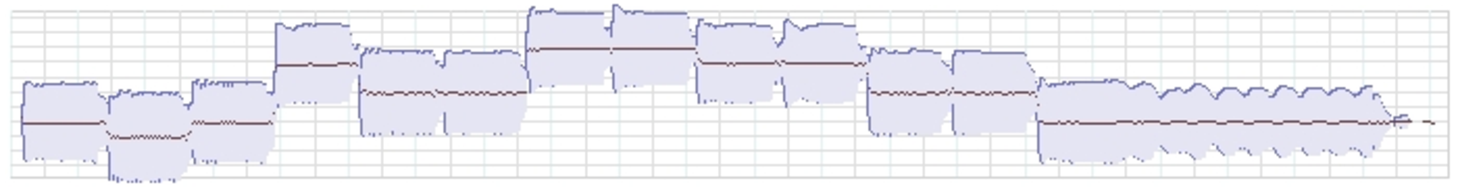
\includegraphics[width=0.99\columnwidth]{rsrc/curves/pitchedarticulation}}
\caption{Pitch and articulation combined.}
\label{fig:pitchedarticulation}
\end{figure}

The corresponding graphic signal is expressed as:
\[ g = S_{f0}\ /\ S_{rms}\ /\ k_c \]
where $S_{f0}$ : fundamental frequency \\
\rshift	 $S_{rms}$ : RMS signal \\
\rshift	 $k_c$ : a constant color signal 
 
%-----------------------------------
\subsubsection{Pitch and harmonics combined}
Combines the fundamental frequency to the first harmonics RMS values
(figure \ref{fig:pitchedstackedharm}). Each harmonic has a different color.
\begin{figure}[htbp]
\centerline{
	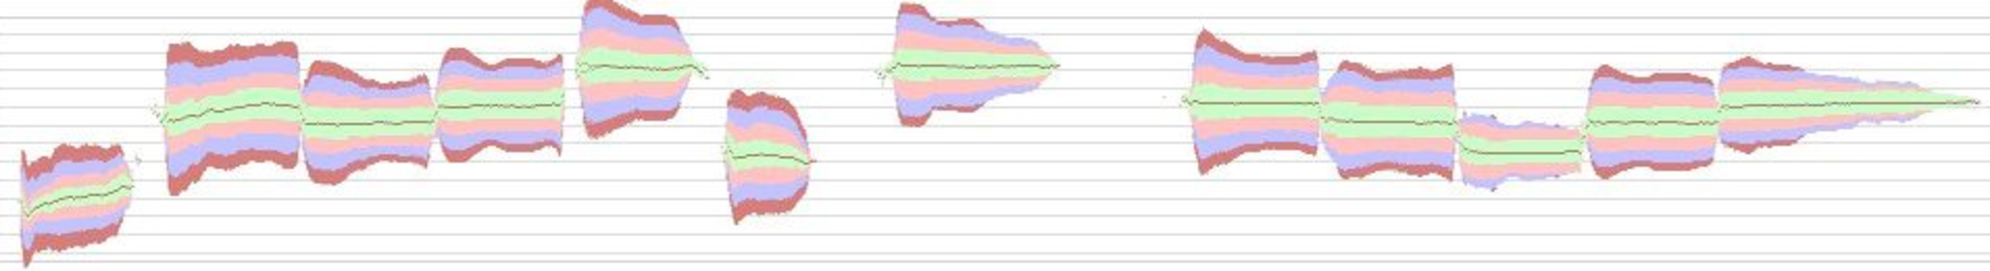
\includegraphics[width=0.99\columnwidth]{rsrc/curves/pitchedstackedharm}}
\caption{Pitch and harmonics combined.}
\label{fig:pitchedstackedharm}
\end{figure}

The graphic signal is described in several steps. First, we build the fundamental frequency graphic as above (see section \ref{pitchart}) :
\[ g0 = S_{f0}\ /\ S_{rms0}\ /\ k_c0 \]
where $S_{f0}$ : fundamental frequency \\
\rshift	 $S_{rms0}$ : f0 RMS values \\
\rshift $k_c0$ : a constant color signal \\
\vspace*{2mm}
Next we build the graphic for the harmonic 1:
\[ g1 = S_{f0} \ /\ S_{rms1} + S_{rms0}\ /\ k_c1 \]
\rshift	 $S_{rms1}$ : harmonic 1 RMS values \\
\rshift $k_c1$ : a constant color signal \\
\vspace{2mm}
Next, the graphic for the harmonic 2:
\[ g2 = S_{f0} /\ S_{rms2} + S_{rms1}  + S_{rms0} \ /\ k_c2 \]
\rshift	 $S_{rms2}$ : harmonic 2 RMS values\\
\rshift $k_c2$ : a constant color signal \\
etc. \\
Finally, the graphic signals are combined into a parallel graphic signal:
\[ g = g2 \ /\  g1 \ /\ g0 \]


%-----------------------------------
\subsection{Interaction}
\label{interact}

\inscore\ is a message driven system that makes use of Open Sound Control [OSC] format. It includes interaction features provided at individual score component level by the way of \emph{watchable events}, which are typical events available in a graphic environment, extended in the temporal domain. The list of supported events is given in table \ref{tblevts}.

\begin{table}[htdp]
\begin{center}
\begin{tabular}{|c|c|c|}
\hline 
mouse events & time events & misc. \\
\hline 
mouse enter	& time enter & new element \\
mouse leave	& time leave &  {\small (at scene level)} \\
mouse down & & \\
mouse up & & \\
mouse move & & \\
double click & & \\
\hline
\end{tabular}
\end{center}
\caption{Typology of \emph{watchable} events.}
\label{tblevts}
\end{table}

Events are associated to user defined messages that are triggered by the event occurrence. The message includes a destination address (\inscore\ by default) that supports a url-like specification, allowing to target any IP host on any UDP port. The message associated to mouse events may use predefined variables, instantiated at event time with the current mouse position or the current position time.

This simple event based mechanism makes easy to describe for example an \emph{intelligent cursor} i.e. an arbitrary object that is synchronized to the score and that turns the page to the next or previous one, depending on the time zone it enters.

%-----------------------------------
\section{\inscore\ messages}
%-----------------------------------
\label{osc}

The \inscore\ API is an OSC messages API. The general format is illustrated in figure \ref{fig:oscformat}: it consists in an address followed by a message string, followed by parameters.

\begin{figure}[htbp]
\centerline{
	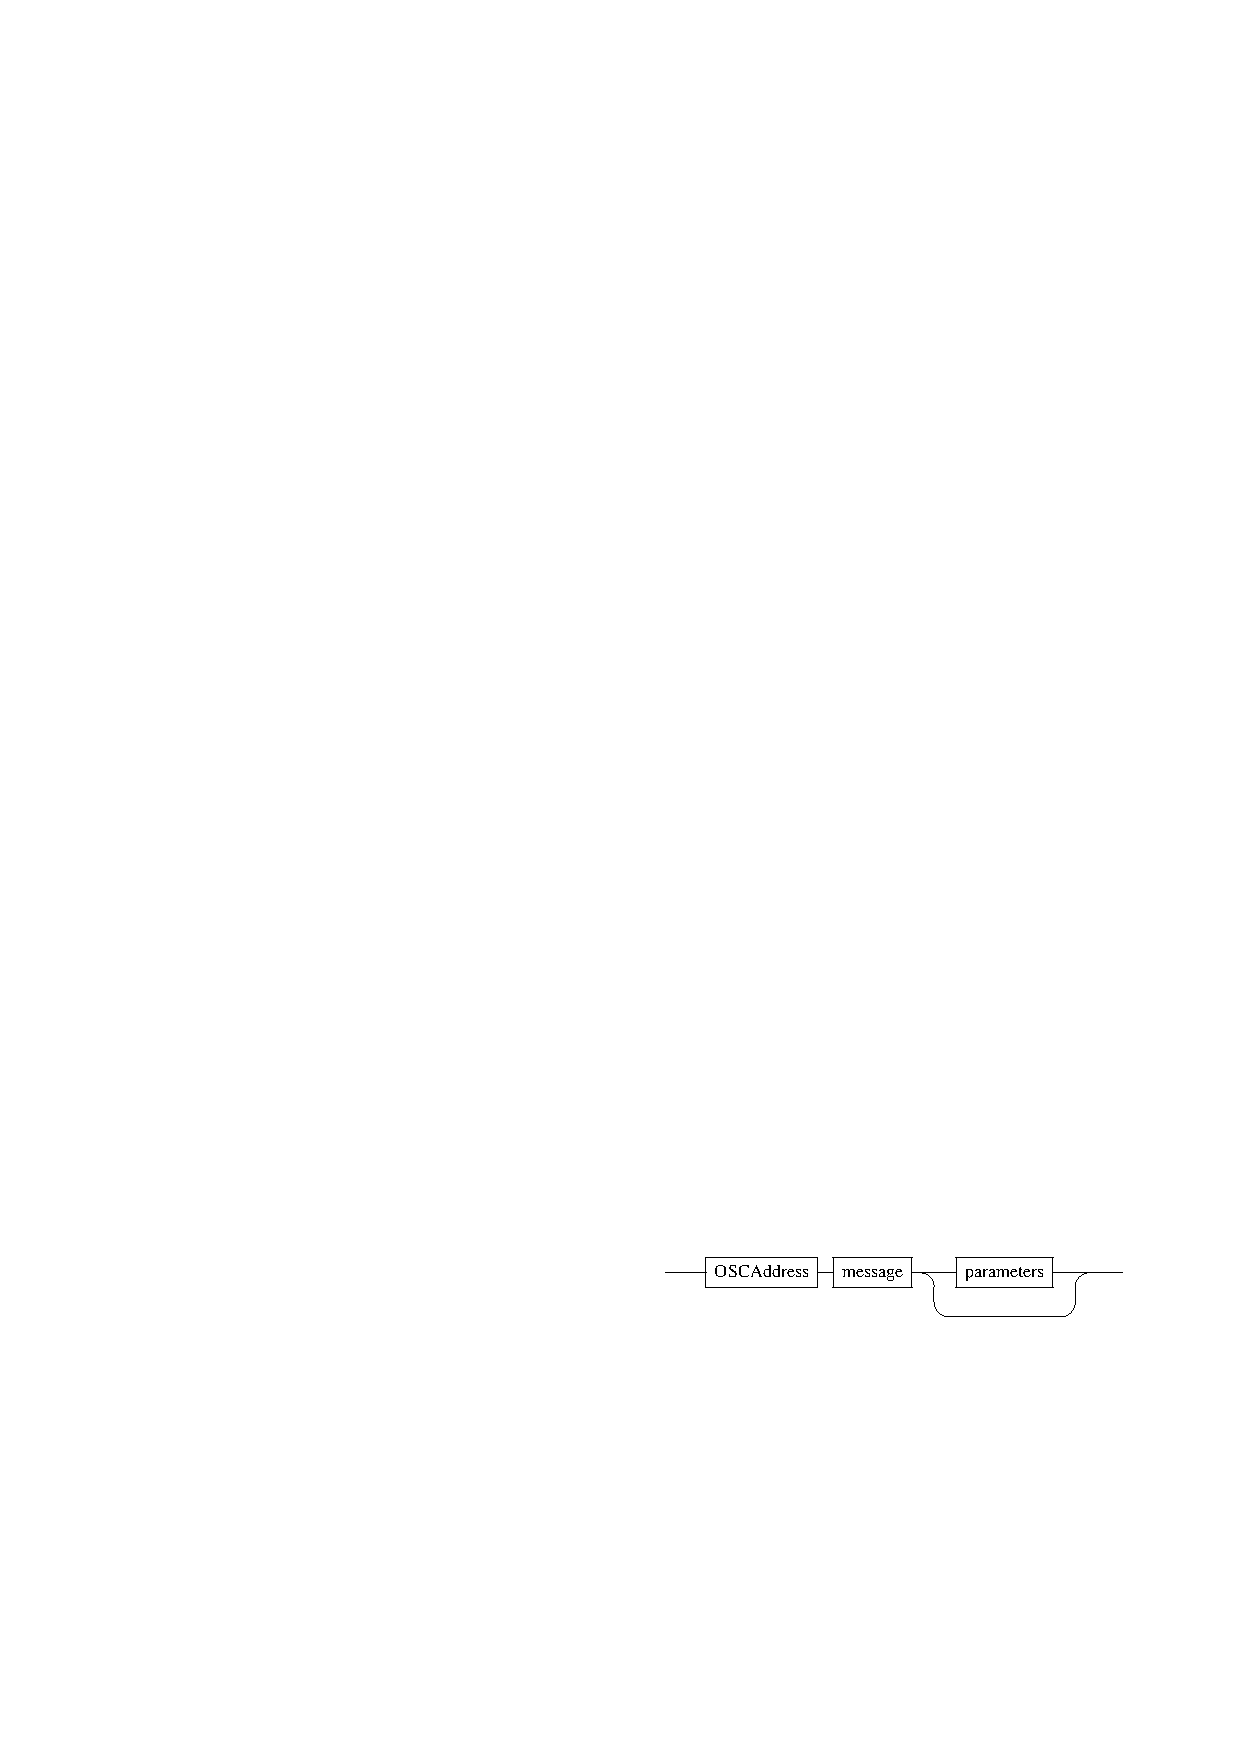
\includegraphics[width=0.99\columnwidth]{rsrc/oscformat}}
\caption{General format of a message.}
\label{fig:oscformat}
\end{figure}

The address may be viewed as an object pointer, the message string as a method name and the parameters as the method parameters. For example, the message:\\
\roshift {\small \texttt{/ITL/scene/score color 255 128 40 150}} \\
may be viewed as the following method call: \\
\roshift {\small \texttt{score->color(255 128 40 150)}}


%-----------------------------------
\subsection{Address space}

The OSC address space is strictly organized like the internal score representation, which is a tree with 4 depths levels (figure \ref{fig:oscaddr}). Messages can be sent to any level of the hierarchy.

The first level is the application level: a static node with a fixed address that is also used to discriminate incoming messages.
An application contains several scenes, which corresponds to different windows and different scores.
Each scene contains components and two static nodes: a $sync$ node for the components synchronization and a $signal$ node, that may be viewed as a special folder containing signals.
The name in blue are user defined, those in black are static reserved names.
\begin{figure}[htbp]
\centerline{
	\includegraphics[width=\columnwidth]{rsrc/oscaddr}}
\caption{\inscore\ address space.}
\label{fig:oscaddr}
\end{figure}


%-----------------------------------
\subsection{Message strings}
\label{oscmsgs}

This section gives some of the main messages supported by all the score components. The list is far from being exhaustive, it is intended to show examples of the system API.

Score components are created and/or modified using a \OSC{set} message (figure \ref{osc:set}) that takes the object type as argument, followed by type specific parameters. 
\begin{figure}[htbp]
\centerline{
	\includegraphics[width=0.6\columnwidth]{rsrc/oscset}}
\caption{The \OSC{set} message.}
\label{osc:set}
\end{figure}

Messages given in figure \ref{osc:pos} are used to set the objects graphic properties.
\begin{figure}[htbp]
\centerline{
	\includegraphics[width=0.7\columnwidth]{rsrc/oscpos}}
\caption{Graphic space management.}
\label{osc:pos}
\end{figure}

Messages given in figure \ref{osc:time} set the time properties. Time is encoded as rational values representing music time (where 1 is a whole note).
\begin{figure}[htbp]
\centerline{
	\includegraphics[width=0.7\columnwidth]{rsrc/osctime}}
\caption{Time management.}
\label{osc:time}
\end{figure}
Graphic space and time management messages have relative positioning forms: the message string prefixed with '\OSC{d}'. 

All the messages that modify the system state have a counterpart \OSC{get} form illustrated by figure \ref{osc:get}.
\begin{figure}[htbp]
\centerline{
	\includegraphics[width=0.8\columnwidth]{rsrc/oscget}}
\caption{Querying the system state.}
\label{osc:get}
\end{figure}

Synchronization between components is based on a master / slave scheme. It is described by a message addressed to the static \OSC{sync} node as illustrated by figure \ref{osc:sync}.
\begin{figure}[h]
\centerline{
	\includegraphics[width=\columnwidth]{rsrc/oscsync}}
\caption{Synchronization message: the second form (2) removes the synchronization from the \OSC{slave} object.}
\label{osc:sync}
\end{figure}
\OSC{syncmode} indicates how to align the slave component to its master: horizontal and/or vertical stretch, etc. 

Interactive features are available by requesting to a component to watch an event using a message like figure \ref{osc:watch}, where \OSC{what} indicates the event (mouseUp, mouseDown, mouseEnter, mouseLeave, timeEnter, timeLeave) and \OSC{OSCMsg} represents any valid OSC message including the address part.
\begin{figure}[htbp]
\centerline{
	\includegraphics[width=0.7\columnwidth]{rsrc/oscwatch}}
\caption{Watching events.}
\label{osc:watch}
\end{figure}

The example in figure \ref{fig:sample} creates a simple score, do some scaling, creates a red cursor and synchronizes it to the score with a vertical stretch to the score height. Output is presented by figure \ref{fig:sampout}.
\begin{figure}[htbp]
\map{/ITL/scene/score  set 'gmn' '[g e f d]';\\
/ITL/scene/score  scale 5.0;\\
/ITL/scene/cursor set 'rect' 0.01 0.1;\\
/ITL/scene/cursor color 255 0 0 150;\\
/ITL/scene/sync 'cursor' 'score' 'v';
}
\caption{\inscore\ sample script.}
\label{fig:sample}
\end{figure}

\begin{figure}[htbp]
\centerline{
	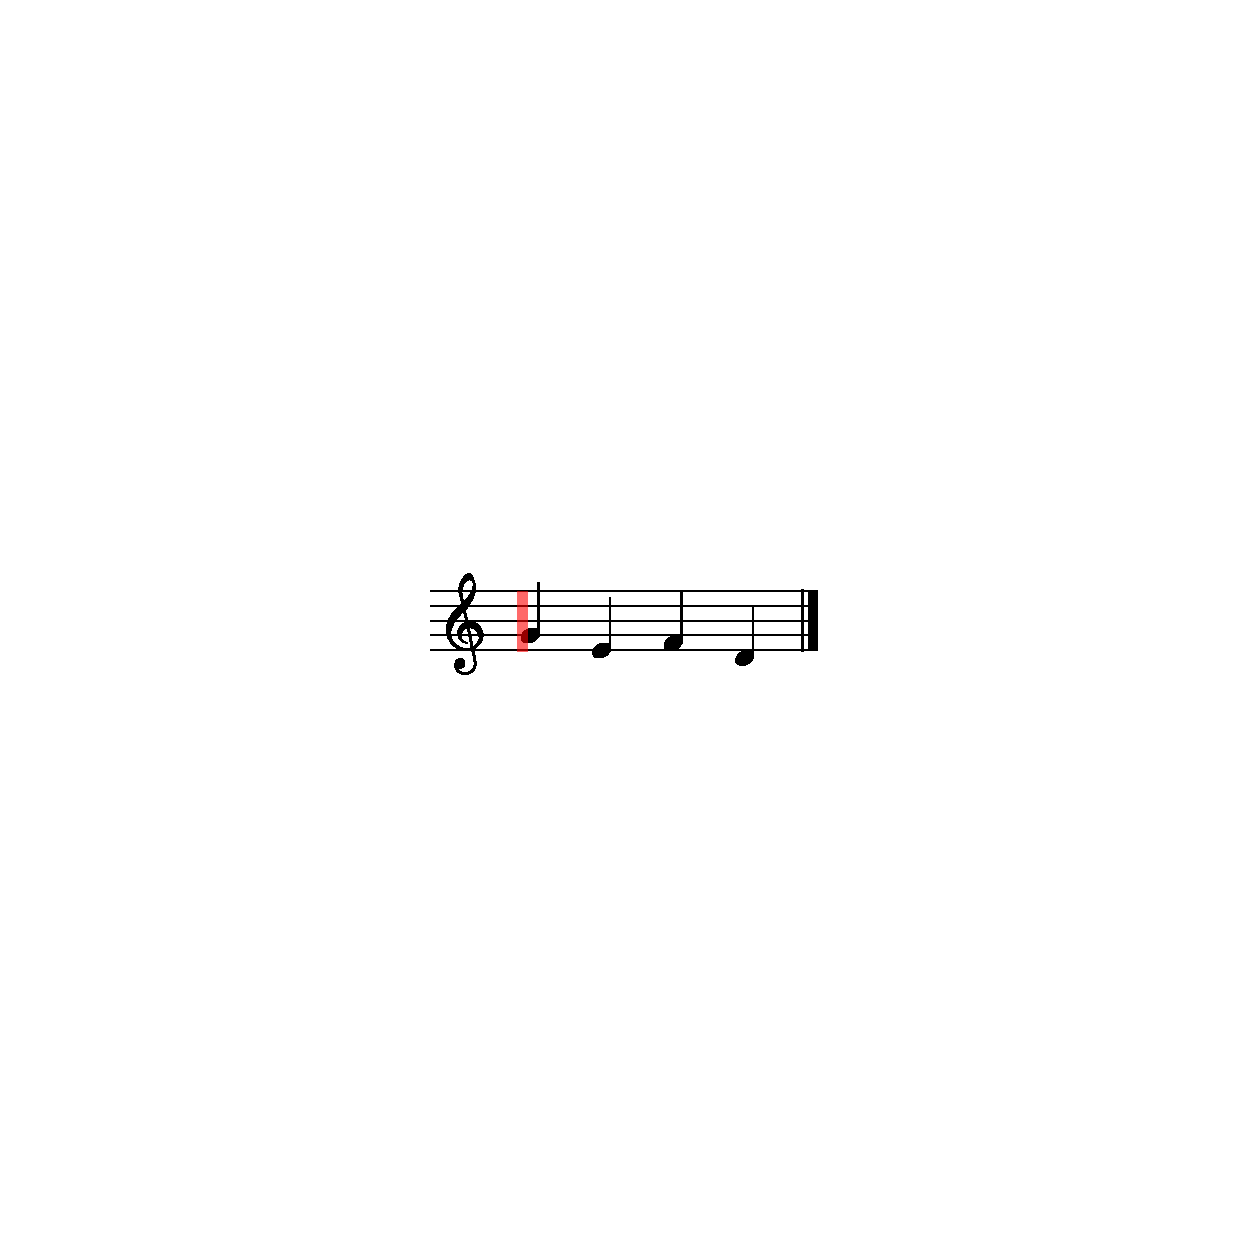
\includegraphics[width=0.6\columnwidth]{rsrc/sample}}
\caption{Sample script output.}
\label{fig:sampout}
\end{figure}


%-----------------------------------
\subsection{\inscore\ scripts}
Actually, the example given in figure \ref{fig:sample}) is making use of the file format of a score, which consists in a list of \emph{textual OSC messages}, separated by a semi-colon. This textual form is particularly suitable to be used as a scripting language and additional support is provided in the form of variables and javascript and/or lua support.

%-----------------------------------
\subsubsection{Variables}

\inscore\ scripts supports variables declarations in the form illustrated by figure \ref{fig:var}. 
\begin{figure}[htbp]
\centerline{
	\includegraphics[width=0.9\columnwidth]{rsrc/oscvar}}
\caption{Variable declaration.}
\label{fig:var}
\end{figure}
Variables may be used in place of any message parameter prefixed using a \$ sign. A variable must be declared before being used.

%-----------------------------------
\subsubsection{Scripting support}
\inscore\ scripts may include javascript sections, delimited by \texttt{<?javascript} and \texttt{?>}
The javascript code is evaluated at parse time. It is expected to produce valid \inscore\ messages as output.
These messages are then expanded in place of the javascript code.

Variables declared before the javascript section are exported to the javascript environment, which make these variables usable in both contexts.

Similarly, \inscore\ may support the lua language in sections delimited by \texttt{<?lua} and \texttt{?>}. By default, lua support is not embedded in the \inscore\ binary distribution. The engine needs to be compiled with the appropriate options to support lua.


%-----------------------------------
\section{Architecture}
%-----------------------------------

\inscore\ is both a shared library and a standalone score viewer application without user interface. Some insight of the system architecture is given in this section for a better understanding and an optimal use of the system. The general architecture is a Model View Controller [MVC] designed to handle OSC message streams. 

%-----------------------------------
\subsection{The MVC Model}

The MVC architecture is illustrated in figure \ref{mvc}. Modification of the model state is achieved by incoming OSC messages or by the library C/C++ API, that is actually also message based. An OSC message is packaged into an \emph{internal messages} representation and stacked on a lock-free fifo stack. These operations are synchronous to the incoming OSC stream and to the library API call. 

\begin{figure}[h]
	\centering 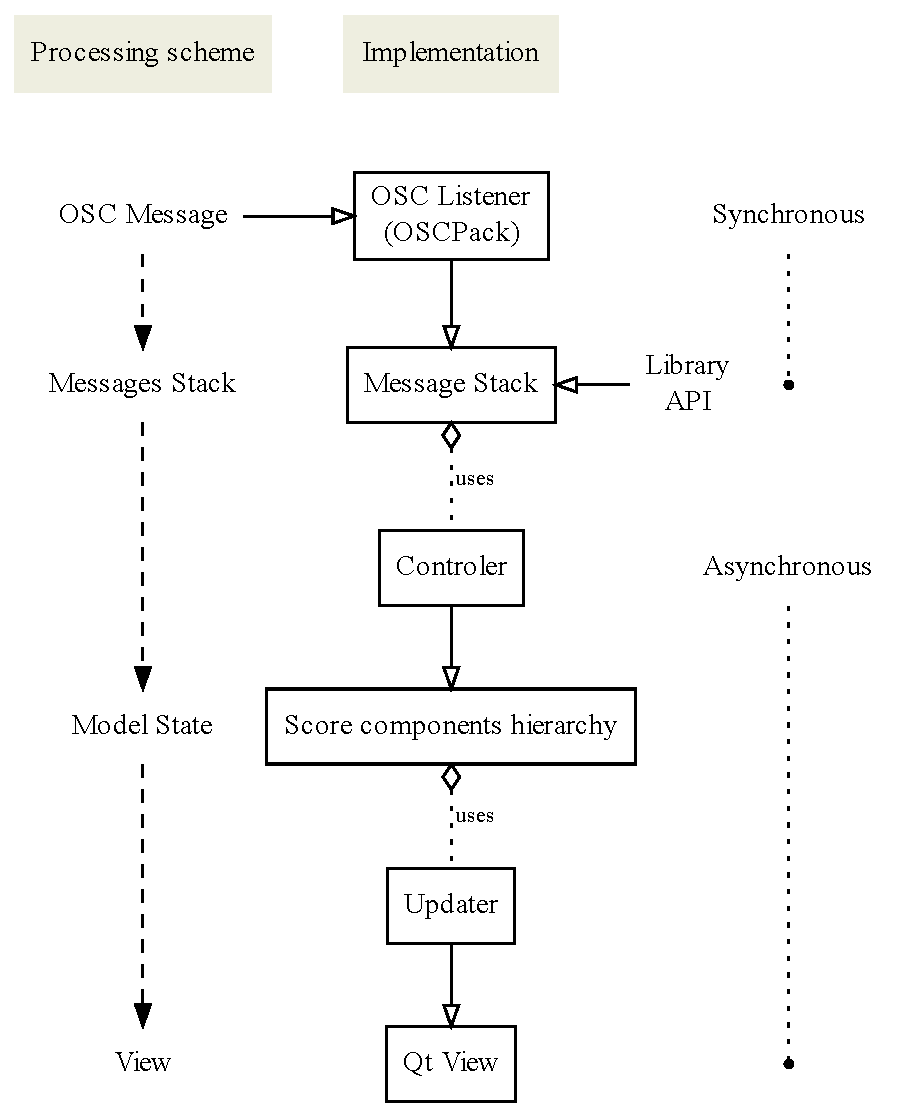
\includegraphics[width=0.98\columnwidth]{rsrc/mvc}
 \caption{An overview of the MVC architecture}
 \label{mvc}
\end{figure}

On a second step, messages are popped from the stack by a \texttt{Controler} that takes in charge address decoding and message passing to the corresponding object of the model. 
The final operation concerns the \emph{view} update. An \texttt{Updater} is in charge of producing a view of the model, which is currently based on the Qt Framework.

This second step of the model modification scheme is asynchronous: it is processed on a regular time base.

 %-----------------------------------
\subsection{Dependencies}

The \inscore\ project depends on external open source libraries:
\begin{itemize}
\item the Qt framework\footnote{\url{http://qt.nokia.com/}} providing the graphic layer and platform independence.
\item the GuidoEngine\footnote{\url{http://guidolib.sourceforge.net}} for music score layout
\item the GuidoQt static library, actually part of the Guido library project
\item the oscpack library\footnote{\url{http://www.rossbencina.com/code/oscpack}} for OSC support
\item and optionally: 
\begin{itemize}
     \item the MusicXML library\footnote{\url{http://libmusicxml.sourceforge.net}}
       to support the MusicXML format.
     \item the v8 javascript engine\footnote{\url{http://code.google.com/p/v8/}} to support javascript in \inscore\ script files.
     \item the lua engine\footnote{\url{http://www.lua.org/}} to support lua in \inscore\ script files.
\end{itemize}
\end{itemize}
The GuidoEngine, the GuidoQt and oscpack libraries are required to compile \inscore.

Binary packages are distributed for Ubuntu Linux, Mac OS and Windows. Detailed instructions are included in the project repository for compiling.


\section{Future work}
Interactive features described in section \ref{interact} result from an experimental approach. The formalization and extension of these features are planned.

Time synchronization features are based on a continuous music time. Supporting other time representations like the Allen relations \cite{Allen:1983:MKT:182.358434} is part of the future work.

Due to its dynamic nature, \inscore\ is particularly suitable to interactive music, i.e. where parts of the music score could be computed in real-time by an interaction system. It could be particularly interesting to provide a musically meaningful visualization of the interaction system state; extensions in this direction are also planned.



\section{Acknowledgements}

\inscore\ was initiated in the Interlude project funded by the French National Research Agency [ANR- 08-CORD-010].


\bibliographystyle{acl}
\bibliography{../interlude}

\end{document}
